%% For normal draft builds (figs undisplayed hence fast compile)
%\documentclass[hyperpdf,nobind,draft,oneside]{hepthesis}
%\documentclass[hyperpdf,nobind,draft,twoside]{hepthesis}

%% For short draft builds (breaks citations by necessity)
%\documentclass[hyperpdf,nobind,draft,hidefrontback]{hepthesis}

%% For Cambridge soft-bound version
\documentclass[hyperpdf,bindnopdf]{hepthesis}
%% For Cambridge hard-bound version (must be one-sided)
%\documentclass[hyperpdf,oneside]{hepthesis}

%% Load special font packages here if you wish
%\usepackage{lmodern}
\usepackage{mathpazo}
%\usepackage{euler}

%% Put package includes etc. into preamble.tex for convenience
\usepackage{graphicx}
\usepackage{xspace}
\usepackage{morefloats,subfig,afterpage}
\usepackage{mathrsfs} % script font
\usepackage{verbatim}
\usepackage{luatex85}
\usepackage[english]{babel}
\selectlanguage{english}
\usepackage[compat=1.1.0]{tikz-feynman}
\usepackage{multirow}
\usepackage{dingbat}
\usepackage{rotating}
%% Using Babel allows other languages to be used and mixed-in easily
%\usepackage[ngerman,english]{babel}

%% Citation system tweaks
\usepackage{cite}
% \let\@OldCite\cite
% \renewcommand{\cite}[1]{\mbox{\!\!\!\@OldCite{#1}}}

%% Maths
% TODO: rework or eliminate maybemath
\usepackage{abmath}
\DeclareRobustCommand{\mymath}[1]{\ensuremath{\maybebmsf{#1}}}
% \DeclareRobustCommand{\parenths}[1]{\mymath{\left({#1}\right)}\xspace}
% \DeclareRobustCommand{\braces}[1]{\mymath{\left\{{#1}\right\}}\xspace}
% \DeclareRobustCommand{\angles}[1]{\mymath{\left\langle{#1}\right\rangle}\xspace}
% \DeclareRobustCommand{\sqbracs}[1]{\mymath{\left[{#1}\right]}\xspace}
% \DeclareRobustCommand{\mods}[1]{\mymath{\left\lvert{#1}\right\rvert}\xspace}
% \DeclareRobustCommand{\modsq}[1]{\mymath{\mods{#1}^2}\xspace}
% \DeclareRobustCommand{\dblmods}[1]{\mymath{\left\lVert{#1}\right\rVert}\xspace}
% \DeclareRobustCommand{\expOf}[1]{\mymath{\exp{\!\parenths{#1}}}\xspace}
% \DeclareRobustCommand{\eexp}[1]{\mymath{e^{#1}}\xspace}
% \DeclareRobustCommand{\plusquad}{\mymath{\oplus}\xspace}
% \DeclareRobustCommand{\logOf}[1]{\mymath{\log\!\parenths{#1}}\xspace}
% \DeclareRobustCommand{\lnOf}[1]{\mymath{\ln\!\parenths{#1}}\xspace}
% \DeclareRobustCommand{\ofOrder}[1]{\mymath{\mathcal{O}\parenths{#1}}\xspace}
% \DeclareRobustCommand{\SOgroup}[1]{\mymath{\mathup{SO}\parenths{#1}}\xspace}
% \DeclareRobustCommand{\SUgroup}[1]{\mymath{\mathup{SU}\parenths{#1}}\xspace}
% \DeclareRobustCommand{\Ugroup}[1]{\mymath{\mathup{U}\parenths{#1}}\xspace}
% \DeclareRobustCommand{\I}[1]{\mymath{\mathrm{i}}\xspace}
% \DeclareRobustCommand{\colvector}[1]{\mymath{\begin{pmatrix}#1\end{pmatrix}}\xspace}
\DeclareRobustCommand{\Rate}{\mymath{\Gamma}\xspace}
\DeclareRobustCommand{\RateOf}[1]{\mymath{\Gamma}\parenths{#1}\xspace}

%% High-energy physics stuff
\usepackage{abhep}
\usepackage{hepnames}
\usepackage{hepunits}
\DeclareRobustCommand{\arXivCode}[1]{arXiv:#1}
\DeclareRobustCommand{\CP}{\ensuremath{\mathcal{CP}}\xspace}
\DeclareRobustCommand{\CPviolation}{\CP-violation\xspace}
\DeclareRobustCommand{\CPv}{\CPviolation}
\DeclareRobustCommand{\LHCb}{LHCb\xspace}
\DeclareRobustCommand{\LHC}{LHC\xspace}
\DeclareRobustCommand{\LEP}{LEP\xspace}
\DeclareRobustCommand{\CERN}{CERN\xspace}
\DeclareRobustCommand{\bphysics}{\Pbottom-physics\xspace}
\DeclareRobustCommand{\bhadron}{\Pbottom-hadron\xspace}
\DeclareRobustCommand{\Bmeson}{\PB-meson\xspace}
\DeclareRobustCommand{\bbaryon}{\Pbottom-baryon\xspace}
\DeclareRobustCommand{\Bdecay}{\PB-decay\xspace}
\DeclareRobustCommand{\bdecay}{\Pbottom-decay\xspace}
\DeclareRobustCommand{\BToKPi}{\HepProcess{ \PB \to \PK \Ppi }\xspace}
\DeclareRobustCommand{\BToPiPi}{\HepProcess{ \PB \to \Ppi \Ppi }\xspace}
\DeclareRobustCommand{\BToKK}{\HepProcess{ \PB \to \PK \PK }\xspace}
\DeclareRobustCommand{\BToRhoPi}{\HepProcess{ \PB \to \Prho \Ppi }\xspace}
\DeclareRobustCommand{\BToRhoRho}{\HepProcess{ \PB \to \Prho \Prho }\xspace}
\DeclareRobustCommand{\X}{\thesismath{X}\xspace}
\DeclareRobustCommand{\Xbar}{\thesismath{\overline{X}}\xspace}
\DeclareRobustCommand{\Xzero}{\HepGenParticle{X}{}{0}\xspace}
\DeclareRobustCommand{\Xzerobar}{\HepGenAntiParticle{X}{}{0}\xspace}
\DeclareRobustCommand{\epluseminus}{\Ppositron\!\Pelectron\xspace}
\DeclareRobustCommand{\protonproton}{\Pproton\APantiproton\xspace}
\DeclareRobustCommand{\ttbar}{\HepProcess{\Pqt \Paqt}\xspace}


%% You can set the line spacing this way
%\setallspacing{double}
%% or a section at a time like this
%\setfrontmatterspacing{double}


%% Define the thesis title and author
\title{A search for dark matter produced in association with \ttbar at \sqrtS=\unit{13}{\TeV} in the dilepton final state with the \CMS experiment} 
\author{Stanislava L. Sevova}

%% Doc-specific PDF metadata
\makeatletter
\@ifpackageloaded{hyperref}{%
\hypersetup{%
  pdftitle = {Search for tt+DM with the CMS detector},
  pdfsubject = {Stanislava Sevova's PhD thesis},
  pdfkeywords = {CMS, Exotics, physics, LHC, heavy flavour},
  pdfauthor = {\textcopyright\ Stanislava Sevova}
}}{}
\makeatother


%% Start the document
\begin{document}

%% Define the un-numbered front matter (cover pages, rubrik and table of contents)
\begin{frontmatter}
  %% Title

\titlepage[\small June 2018]{}%  A dissertation submitted to Northwestern University\\ for the degree of Doctor of Philosophy}

%% Abstract
\begin{abstract}%[\smaller \thetitle\\ \vspace*{1cm} \smaller {\theauthor}]
  %\thispagestyle{empty}
  A vast portion of the Universe is predicted to consist of an as-of-yet undetected, non-luminous form of matter, known as dark matter. Evidence of its existence has been corroborated by various astrophysical observations at many cosmological scales, and its relative abundance has been determined. However, knowledge of its nature and non-gravitational interactions is entireley lacking. Nonetheless, the predicted particle nature of dark matter allows for multiple complementary methods of its detection.

This work presents a search for dark matter produced in association with a top quark pair performed using the data recorded by the CMS detector at the LHC in Geneva, Switzerland during 2016. The collision center-of-mass energy of the dataset in question is 13\:\TeV, and the integrated luminosity of the dataset corresponds to $35.9\:\textrm{fb}^{-1}$. The analysis performed considers only the dilepton decay of top quark pairs. The results are interpreted using simplified models of dark matter and are compared to corresponding results from direct detection experiments. While the work does not provide evidence of the production of dark matter in association with a top quark pair in the dilepton final state from proton-proton collisions, it sets important constraints on the properties of dark matter. 
\end{abstract}


%% Declaration
\begin{declaration}
        The following dissertation is the result of my own work conducted while based at Northwestern University and CERN. Explicit references are made to acknowledge the work of others. This dissertation has not been submitted for another qualification to Northwestern University or any other university.
  \vspace*{1cm}
  \begin{flushright}
    Stanislava Sevova
  \end{flushright}
\vspace*{\fill}
\begin{center}
\copyright\:Copyright by Stanislava Sevova 2018 \\
All Rights Reserved
\end{center}

\end{declaration}


%% Acknowledgements
\begin{acknowledgements}

A great number of people deserve recognition for directly or indirectly providing me with the support required to complete this work. Of particular prominence are my advisor at Northwestern, Kristian Hahn, and the post-doctoral researcher who has provided invaluable mentorship since day one, Kevin Sung. I would like to thank Kristian for his strong leadership and constant support of my research as a graduate student. His guidance and creativity have only amplified my own passion for particle physics throughout the years, and it has truly been a rewarding experience to work with him. To Kevin, I owe an immense amount of gratitude for his patience, understanding, and attention to detail. I have been extremely fortunate to learn from someone as knowledgeable and precise as Kevin, and I am beyond grateful for all the help he has provided over the years! I will especially and genuinely miss the office camaraderie. In addition, I would like to thank other excellent CMS colleagues, Phil Harris, Nhan Tran, and Marco Trovato who provided additional support and interesting research opportunities for me to pursue.

Throughout my graduate career, I was lucky to be surrounded by a wonderful group of friends both in Chicago and Geneva, a few of whom I feel should be mentioned by name. I would like to thank my dear friend Mary Crofton for her constant ability to take my mind off research with fun activities, and also for giving me a place to stay and feeding me while in Chicago! I would like to thank my friends Rickard Strom, Sophie Baker, and Andrew Carnes for imparting a bit of their undying sense of adventure onto me, and for the laughs they always provide. Finally, I would like to thank Leonora Vesterbacka for always being there, always knowing what to say, and always having my back! I will cherish our friendship for life. 

I would be remiss if I did not acknowledge how much Doug Schaefer has rejuvenated my quality of life in recent months, and would like to thank him not only for his immense support in recent weeks, but also for the joy he has provided me in all of our adventures together, big or small. 

To conclude, above all I am deeply thankful to my family. To my younger sister, Ralitza, I am thankful for all the ways you are able to make me smile, and I truly cherish your youthful wisdom! I look forward to giving you the same love and support you've provided me with, as you reach new heights. I dedicate this work to my parents, Penka and Lubomir, to whom I cannot express in enough words how grateful I am. You have taught me to follow my passions, persevere through the obstacles, and never be afraid of the unknown. Your support is eternal, as is my love for you. Thank you.
                        
        
%  Of the many people who deserve thanks, some are particularly prominent,
%  such as my supervisor\dots
\end{acknowledgements}


%% Preface
%\begin{preface}
%        This thesis describes my research on various aspects of the \CMS particle physics program, centred around the \CMS detector and \LHC accelerator at \CERN in Geneva.
%
%  \noindent
%  For this example, I'll just mention \ChapterRef{chap:SomeStuff}
%  and \ChapterRef{chap:MoreStuff}.
%\end{preface}

%% ToC
\tableofcontents


%% Strictly optional!
%\frontquote{%
%  Writing in English is the most ingenious torture\\
%  ever devised for sins committed in previous lives.}%
%  {James Joyce}
%% I don't want a page number on the following blank page either.
\thispagestyle{empty}

\end{frontmatter}

%% Start the content body of the thesis
\begin{mainmatter}
  %% Actually, more semantic chapter filenames are better, like "chap-bgtheory.tex"
  \chapter{Dark matter: Beyond the Standard Model}
\label{chap:DM}

%% Restart the numbering to make sure that this is definitely page #1!
\pagenumbering{arabic}

%% Note that the citations in this chapter use the journal and
%% arXiv keys: I used the SLAC-SPIRES online BibTeX retriever
%% to build my bibliography. There are also quite a few non-standard
%% macros, which come from my personal collection. You can have them
%% if you want, or I might get round to properly releasing them at
%% some point myself.

The Standard Model (SM) of particle physics, although an extremely successful theory encoding the properties of elementary particles and their interactions, has its deficiencies. For one, cosmological and astrophysical observations supply compelling evidence~\cite{Bertone:2004pz, Feng:2010gw, Porter:2011nv} for the existence of dark matter (DM), a piece of the astro-particle physics puzzle which does not fit in with the SM. 
%~\cite{Phys.Rev.Lett.19.1264, Phys.Rev.D2.1285,hep-ph/0410370}.


  \chapter{The \CMS experiment}
\label{chap:MoreStuff}

%\chapterquote{There, sir! that is the perfection of vessels!}
%{Jules Verne, 1828--1905}

\section{The \LHC}
The Large Hadron Collider (\LHC) at \CERN is the most powerful particle accelerator in the world, located in the same tunnel as the Large Electron-Positron collider (\LEP)~\cite{Brianti:2004qq}. The mandate of the \LHC experimental program is two-fold: to probe the electroweak symmetry breaking mechanism via which particles in the Standard Model (SM) attain mass, and to explore an energy frontier in the search for new physics beyond the SM (\BSM).

\section{The \CMS experiment}
\label{sec:CMSInDetail}

%Since both \bhadron{s} are preferentially produced in the same direction
%and are forward-boosted along the beam-pipe, the detector is not required
%to have full $4\pi$ solid-angle coverage. \LHCb takes advantage of this
%by using a wedge-shaped single-arm detector with angular acceptance
%\unit{10-300}{\mrad} in the horizontal (bending) plane~\cite{Amato:1998xt}.

\vspace{1cm}

\begin{center}
{\hspace{1mm}\Large\vdots\hspace{1cm}}
\end{center}

\vspace{1cm}

The detector is illustrated in \FigureRef{fig:LHCbCrossSection}, showing
the overall scale of the experiment and the surrounding cavern structure.
%
%\begin{sidewaysfigure}
%  \begin{center}
%  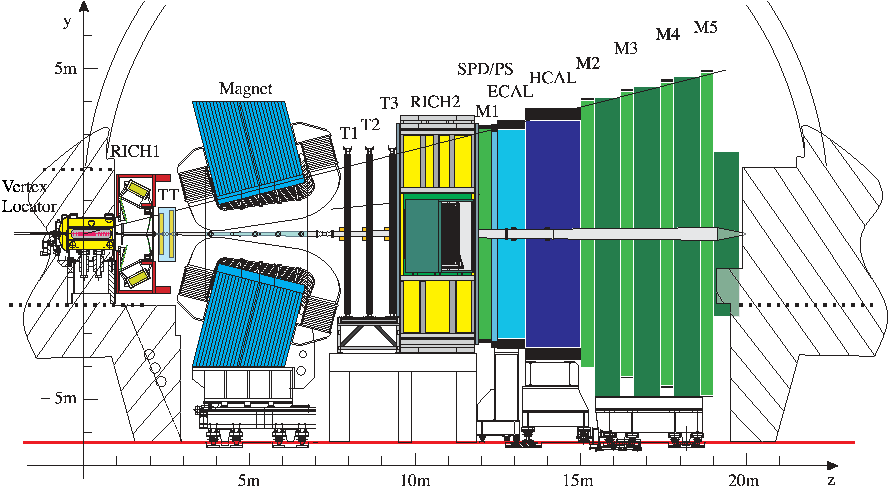
\includegraphics[width=0.8\textheight]{lhcb-detector-cross-section.pdf}
%  \caption[Cross-section view of \LHCb, cut in the non-bending $y$--$z$ plane]%
%    {Cross-section view of \LHCb, cut in the non-bending $y$--$z$ plane.}
%  \label{fig:LHCbCrossSection}
%  \end{center}
%\end{sidewaysfigure}

The single-sided detector design was chosen in preference to a two-armed
design since the detector dimensions are restricted by the layout of the
IP8 (ex-Delphi) cavern in which \LHCb is located. Using all the available
space for a single-arm spectrometer more than compensates in performance
for the \about{50\percent} drop in luminosity.

\section{The \Cerenkov mechanism}
A Huygens construction in terms of spherical shells of probability for photon
emission as the particle progresses along its track shows an effective
``shock-front'' of \Cerenkov emission. This corresponds to an emission cone of
opening angle \thetaCerenkov around the momentum vector for each point on the
track,
%
\begin{subequations}
  \label{eq:cosThetaCk}
  \begin{equation}
    \cos\,\thetaCerenkov  &= \frac{1}{n \beta} +
                             \frac{\hbar k}{2p}%
                             \parenths{ 1 - \frac{1}{n^2} } \\
                          &\,\sim \frac{1}{n \beta}%
    \label{eq:cosThetaCkApprox}
  \end{equation}
\end{subequations}
%
where $\beta \equiv v/c$, the relativistic velocity fraction.

\section{Trigger system}
\label{sec:triggers}
An overview of the \LHCb trigger characteristics broken down by level
is shown in \Table~\ref{tab:TriggerDetails}.

\begin{table}[bp]
  \begin{tabular}{lllll}
                & L0              & L1              & HLT             \\
    \midrule\\
    Input rate  & \unit{40}{\MHz} & \unit{1}{\MHz}  & \unit{40}{\kHz} \\
    Output rate & \unit{1}{\MHz}  & \unit{40}{\kHz} & \unit{2}{\kHz}  \\
    Location    & On detector     & Counting room   & Counting room   \\
  \end{tabular}
  \caption{Characteristics of the trigger levels and offline analysis.}
  \label{tab:TriggerDetails}
\end{table}

  \chapter{Continued captions}
\label{chap:ContCaptions}

Here are some funky floats using ``continued captions'', i.e. for a semantically
collected group of float contents which are too numerous to fit into a single
float, such as the pretty circles in the following figure:

\newcommand{\circleimg}[1]{%
\begin{tikzpicture}
  \draw[color=black,fill=#1,thick] (1,0) circle (1.5cm);
\end{tikzpicture}%
}

\begin{figure}[hb]
  \subfloat[][Example 1a]{\label{fig:cc1a}\circleimg{red!80}}\quad
  \subfloat[][Example 1b]{\label{fig:cc1b}\circleimg{green!70!yellow}}\quad
  \subfloat[][Example 1c]{\label{fig:cc1c}\circleimg{blue!80}}\quad
  \subfloat[][Example 1d]{\label{fig:cc1d}\circleimg{orange!80!yellow}}
  \caption{Demonstration of \texttt{subfig} continued captions.}
  \label{fig:cc1}
\end{figure}

\begin{figure}[p]
  \ContinuedFloat
  \subfloat[][Example 1e]{\label{fig:cc1e}\circleimg{violet}}\quad
  \subfloat[][Example 1f]{\label{fig:cc1f}\circleimg{cyan}}\quad
  \subfloat[][Example 1g]{\label{fig:cc1g}\circleimg{magenta}}\quad
  \subfloat[][Example 1h]{\label{fig:cc1h}\circleimg{yellow}}
  \caption[]{Demonstration of \texttt{subfig} continued captions (continued).}
\end{figure}

\noindent
This mechanism means that the same float label is used for both pages of
floats. Note that we can refer to \FigureRef{fig:cc1} in general, or to
\FigureRef{fig:cc1g} on \PageRef{fig:cc1g} in particular!

\noindent
Just for the hell of it, let's also refer to \SectionRef{sec:neutralmixing}.

  %% To ignore a specific chapter while working on another, making the build faster, comment it out:
  %\input{chap4}
\end{mainmatter}

%% Produce the appendices
\begin{appendices}
  %% The "\appendix" call has already been made in the declaration
%% of the "appendices" environment (see thesis.tex).
\chapter{Pointless extras}
\label{app:Pointless}

\chapterquote{%
Le savant n'\'etudie pas la nature parce que cela est utile; \\
\indent il l'\'etudie parce qu'il y prend plaisir, \\
\indent et il y prend plaisir parce qu'elle est belle.}%
{Henri Poincar\'e, 1854--1912}

Appendixes (or should that be ``appendices''?) make you look really clever, 'cos
it's like you had more clever stuff to say than could be fitted into the main
bit of your thesis. Yeah. So everyone should have at least three of them\dots

\section{Like, duh}
\label{sec:Duh}
Padding? What do you mean?

\section{$y = \alpha x^2$}
\label{sec:EqnTitle}
See, maths in titles automatically goes bold where it should (and check the
table of contents: it \emph{isn't} bold there!) Check the source: nothing
needs to be specified to make this work. Thanks to Donald Arsenau for the
teeny hack that makes this work.

%% Big appendixes should be split off into separate files, just like chapters
%\input{app-myreallybigappendix}

\end{appendices}

%% Produce the un-numbered back matter (e.g. colophon,
%% bibliography, tables of figures etc., index...)
\begin{backmatter}
  \begin{colophon}
  This thesis was made in \LaTeXe{} using the ``hepthesis'' class~\cite{hepthesis}.
\end{colophon}

%% You're recommended to use the eprint-aware biblio styles which
%% can be obtained from e.g. www.arxiv.org. The file mythesis.bib
%% is derived from the source using the SPIRES Bibtex service.
\bibliographystyle{h-physrev}
\bibliography{mythesis}

%% I prefer to put these tables here rather than making the
%% front matter seemingly interminable. No-one cares, anyway!
\listoffigures
\listoftables

%% If you have time and interest to generate a (decent) index,
%% then you've clearly spent more time on the write-up than the
%% research ;-)
%\printindex

\end{backmatter}

%% Close
\end{document}
